%%%%%%%%%%%%%%%%%%%%%%%%%%%%%%%%%%%%%%%%%%%%%%%%%%%%%%%%%%%%%%%%%%%%%%%%%%%%%%%%%%%%%%%%%%
%%
%% Description:		This is an example presentation using the beamerthemedhbw
%%
%%					The beamerthemedhbw is based on jacksbeamertheme
%%					(https://github.com/JacknJo/jacksbeamertheme)
%%
%% Author:			Hannes Bartle																				
%% 					DHBW Ravensburg Campus Friedrichshafen		
%%					September 2016	
%% 
%% The beamerthemedhbw is free software: you can redistribute it and/or modify
%% it under the terms of the GNU General Public License as published by
%% the Free Software Foundation, either version 3 of the License, or
%% (at your option) any later version.
%% 
%% The beamerthemedhbw is distributed in the hope that it will be useful,
%% but WITHOUT ANY WARRANTY; without even the implied warranty of
%% MERCHANTABILITY or FITNESS FOR A PARTICULAR PURPOSE.  See the
%% GNU General Public License for more details.
%% 
%% You should have received a copy of the GNU General Public License
%% along with the beamerthemedhbw.  If not, see <http://www.gnu.org/licenses/>.
%% 
%% 
%%%%%%%%%%%%%%%%%%%%%%%%%%%%%%%%%%%%%%%%%%%%%%%%%%%%%%%%%%%%%%%%%%%%%%%%%%%%%%%%%%%%%%%%%%


\documentclass[	12pt, 				
				t,					
				aspectratio=169,
				%handout-PLACEHOLDER
				]{beamer}

\usepackage{dhbwstyle}

\title{Listenstrukturen}

\begin{document}
	
	\begin{frame}[noframenumbering]
		\titlepage
	\end{frame}


	\begin{frame}[allowframebreaks]{Inhalt}
		\tableofcontents
	\end{frame}
	
	\outlineFrame{Allgemeines}
	\begin{frame}{Multithreading}{Allgemeines (Vgl. \cite{ullenboom2018java} S. 948)}
    \begin{itemize}
        \item Moderne Betriebssysteme unterstützen \textit{Multitasking}
        \item Bedeutet: Mehrere Programme können gleichzeitig laufen
        \item Man spricht in der Regel von \textit{Nebenläufigkeit}
        \item Wie diese erreicht wird steuert das Betriebssystem (und ggf. Hardware)
        \item Auf Mehrkernprozessoren können "`echt parallel"' arbeiten
        \item Auf Einkernsystemen wird eine Parallelität "`simulisert"' (\textit{Quasiparallelität})
    \end{itemize}
\end{frame}

\begin{frame}{Multithreading}{Technische Umsetzung (Vgl. \cite{ullenboom2018java} S. 948)}
    \begin{itemize}
        \item Jeder Prozessorkern kann (in der Regel) zu einem Zeitpunkt einen Prozess bearbeiten
        \item In der Regel gibt es deutlich mehr laufende Prozesse als Kerne
        \item Lösung: Aktiver Prozess wird auf den Kernen hochfrequent (im Millisekundenbereich) umgeschalten
        \item Umschaltung erfolgt durch den \textit{Scheduler}
        \item Zur Umschaltung der Prozesse gibt es diverse Strategien mit diversen Parametern:
        \begin{itemize}
            \item Priorität
            \item Bearbeitungsdauer
            \item "`Fail-Count"' -- Wie oft wurde der Prozess schon versucht zu bearbeiten
        \end{itemize}
    \end{itemize}
\end{frame}

\begin{frame}{Prozesse}{Grundlegende Eigenschaften (Vgl. \cite{ullenboom2018java} S. 948)}
    \begin{itemize}
        \item Jeder Prozess besteht im Grunde aus:
        \begin{itemize}
            \item Dem auszuführenden Programmcode
            \item Den dazugehörigen Daten
            \item Einem \textit{eigenen} (isolierten) Speicherbereich
            \item Ggf. Verwendete Ressourcen wie Dateien oder Laufwerke
        \end{itemize}
        \item Durch die Trennung des Speicherbereichs können Prozesse nicht auf die Daten anderer Prozesse zugreifen!
        \item Ist doch ein Datenaustausch zwischen Prozessen erforderlich, ist ein spezielle \textit{Shared Memory} Bereich notwendig
        \item Prozesse können aus mehreren parallelen Threads bestehen $\rightarrow$ Diese können die gleichen Ressourcen nutzen
    \end{itemize}
\end{frame}

\begin{frame}{Nebenläufigkeit}{Geschwindigkeitsgewinn (Vgl. \cite{ullenboom2018java} S. 949ff)}
    \begin{itemize}
        \item Nebenläufigkeit führt in der Regel zu Geschwindigkeitsgewinn
        \item In Mehrkernsystemen sowieso...
        \item ...aber auch in Einkernsystemen
        \item Beispiel: Software zur Erstellung von Datenbank-Reports:
        \begin{itemize}
            \item Baue ein Fenster auf
            \item Öffnen der Datenbank vom Server, lesen der Datensätze
            \item Analyse der Daten, Visualisierung des Fortschritts
            \item Datei öffnen, Analyseergebnisse in Datei schreiben
        \end{itemize}
    \end{itemize}
\end{frame}

\begin{frame}{Nebenläufigkeit}{Beispiel für Geschwindigkeitsgewinn (Vgl. \cite{ullenboom2018java} S. 949ff)}
    \begin{itemize}
        \item Betrachten wir einmal die parallelisierbaren Abschnitte:
        \begin{itemize}
            \item Öffnen von Fenster und Datenbank können parallel geschehen
            \item Lesen neuer Datensätze und Analyse alter Datensätze kann parallel erfolgen
            \item Analyse neuer Datensätze und schreiben von alten analysierten Daten kann gleichzeitig abgearbeitet werden
        \end{itemize}
        \item Hier auch auf einem Einprozessorsystem großer Leistungsgewinn
        \item Da die parallelen Prozesse verschiedene \textit{Ressourcen} belasten
    \end{itemize}
\end{frame}

\begin{frame}{Nebenläufigkeit}{Beispiel für Geschwindigkeitsgewinn (Vgl. \cite{ullenboom2018java} S. 949ff)}
    \begin{itemize}
        \item Während auf das Fertigstellen einer Ressource gewartet wird, können Aufgaben bearbeitet werden die andere Ressourcen benötigen:
        \begin{itemize}
            \item Während der Prozessor ausgelastet ist die GUI zu erstellen kann eine Datei auf der Festplatte geöffnet werden $\rightarrow$ Dateioperationen benötigen wenig Prozessorleistung, eher durch Festplattengeschwindigkeit begrenzt
            \item Während Daten z.B. aus einer Datenbank abgerufen werden wird hauptsächlich die Netzwerkressource belastet $\rightarrow$ Prozessorleistung kann ggf. anders genutzt werden
            \item Parallel zu einer Prozessorlastigen Analyse können bereits analysierte Daten in eine Datei geschrieben werden
        \end{itemize}
        \item Kurz gesagt: Wir nutzen "`Wartezeiten"' von langsamen Operationen zu unserem Vorteil
    \end{itemize}
\end{frame}

\begin{frame}{Nebenläufigkeit}{Fazit (Siehe \cite{ullenboom2018java} S. 951)}
    \begin{itemize}
        \item Nebenläufigkeit muss gut geplant werden
        \item Insbesondere für Einkernsysteme
        \item Geschwindigkeitsgewinn nur vorhanden, wenn die parallelen Aktivitäten unterschiedliche Ressourcen nutzen
        \item Durch Nebenläufigkeit entsteht auch ggf. zusätzlicher Overhead für Synchronisation
        \item Zum Beispiel, wenn auf ein Teilergebnis gewartet werden muss
        \item Hier muss insbesondere auf konkurrierende Zugriffe und gegenseitige Wartebedingungen geachtet werden, um \textit{Deadlocks} zu vermeiden
    \end{itemize}
\end{frame}


	
	\outlineFrame{Arrays}
	\begin{frame}{Allgemeines}{Über Arrays}
	\begin{itemize}
		\item Einfachste Listenstruktur
		\item Speichert Daten sequentiell im Speicher
		\item In der Regel nur in einer Dimension
		\item Aber auch "`mehrdimensionale"' Arrays möglich
		\item Logisch (und auch vom Zugriff) könnte man Arrays vergleichen mit:
		\begin{itemize}
			\item Vektoren bei eindimensionalen Arrays
			\item Matrizen für zwei- oder höherdimensionale Arrays
		\end{itemize}
	\end{itemize}
\end{frame}

\begin{frame}{Eigenschaften}{Von Arrays}
	\begin{itemize}
		\item Belegen einen fortlaufenden Bereich im Speicher
		\item Dadurch:
		\begin{itemize}
			\item Muss die Größe bei Initialisierung bekannt sein
			\item Sind Zugriffe auf die Elemente sehr schnell
			\item Löschen-/Einfügen von Elementen jedoch vergleichsweise "`teuer"'
		\end{itemize}
		\item Technisch ist ein Array meist lediglich ein Zeiger auf den Beginn des Arrays
		\item Arrays sind meist für Datenmengen mit vielen Elementen(Ab ~65535) ungeeignet
		\item Warum?
	\end{itemize}
\end{frame}

\begin{frame}{Datenstruktur von Arrays}{Bildlich dargestellt}
	\begin{figure}
		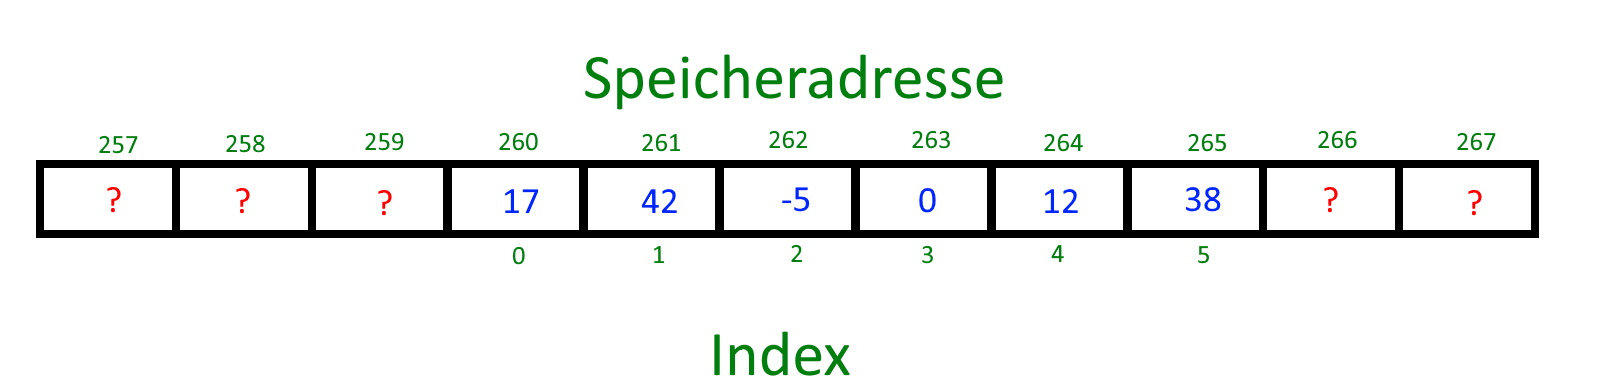
\includegraphics[width=\textwidth]{graph/Array_base}
	\end{figure}
\end{frame}

\begin{frame}{Grundoperationen}{Anlegen eines Arrays}
	\begin{itemize}
		\item Bei Anlegen eines Arrays muss immer die Größe festgelegt werden
		\item Vorher können keine Elemente hinzugefügt bzw. manipuliert werden
		\item Bei Initialisierung des Arrays wird ein Speicherbereich für dieses reserviert
		\item Größe des Speicherbereichs für ein Array der Größe $N$ ergibt sich aus:
	\end{itemize}
	$Speicher_{Byte}=ElementSize_{Byte}\cdot N$
\end{frame}

\begin{frame}{Grundoperationen}{Zugriff auf Elemente}
	\begin{itemize}
		\item Zugriffe auf Listenelemente passieren immer in konstanter Zeit
		\item Dadurch ergibt sich die Komplexität zu: $O(1)$
		\item Begründung:
		\begin{itemize}
			\item Elemente liegen "`hintereinander"' im Speicher $\rightarrow$ Haben fortlaufende Speicheradressen
			\item Die Adresse des ersten Elements ist immer bekannt
			\item Heißt, bei Abrufen des $n$-ten Elements muss von der Startadresse nur eine bestimmte Schrittzahl addiert werden
			\item Jeder Zugriff auf ein Element ist somit (auf unterster Ebene) eine Addition und eine Leseoperation
		\end{itemize}
	\end{itemize}
\end{frame}


\begin{frame}{Graphische Darstellung}{Zugriff auf Elemente}
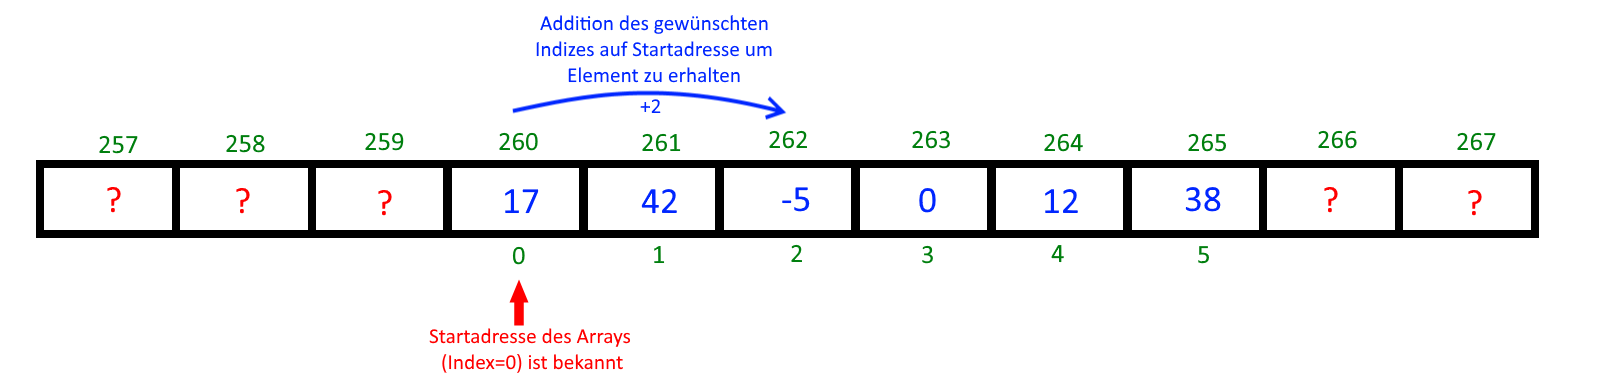
\includegraphics[width=\textwidth]{graph/array_access}
\end{frame}

\begin{frame}{Grundoperationen}{An-/Einfügen von Elementen}
	\begin{itemize}
		\item Nachträgliches Einfügen von Elementen ist nicht trivial
		\item Grund dafür ist die Speicherstruktur von Arrays
		\item Dadurch, dass die Elemente fortlaufend im Speicher liegen...
		\begin{itemize}
			\item ...müsste bei Einfügen sichergestellt sein, dass der nachfolgende Speicher noch nicht genutzt ist (Was meist nicht der Fall ist)
			\item ...und alle Elemente die nach dem eingefügten Element liegen, nach rechts "`verschoben"' werden
		\end{itemize}
		\item Dadurch häufig das anlegen eines neuen Arrays nötig
		\item Und das ausführen von vielen Kopieroperationen
	\end{itemize}
\end{frame}

\begin{frame}{Einfügen in Arrays}{Visualisiert}
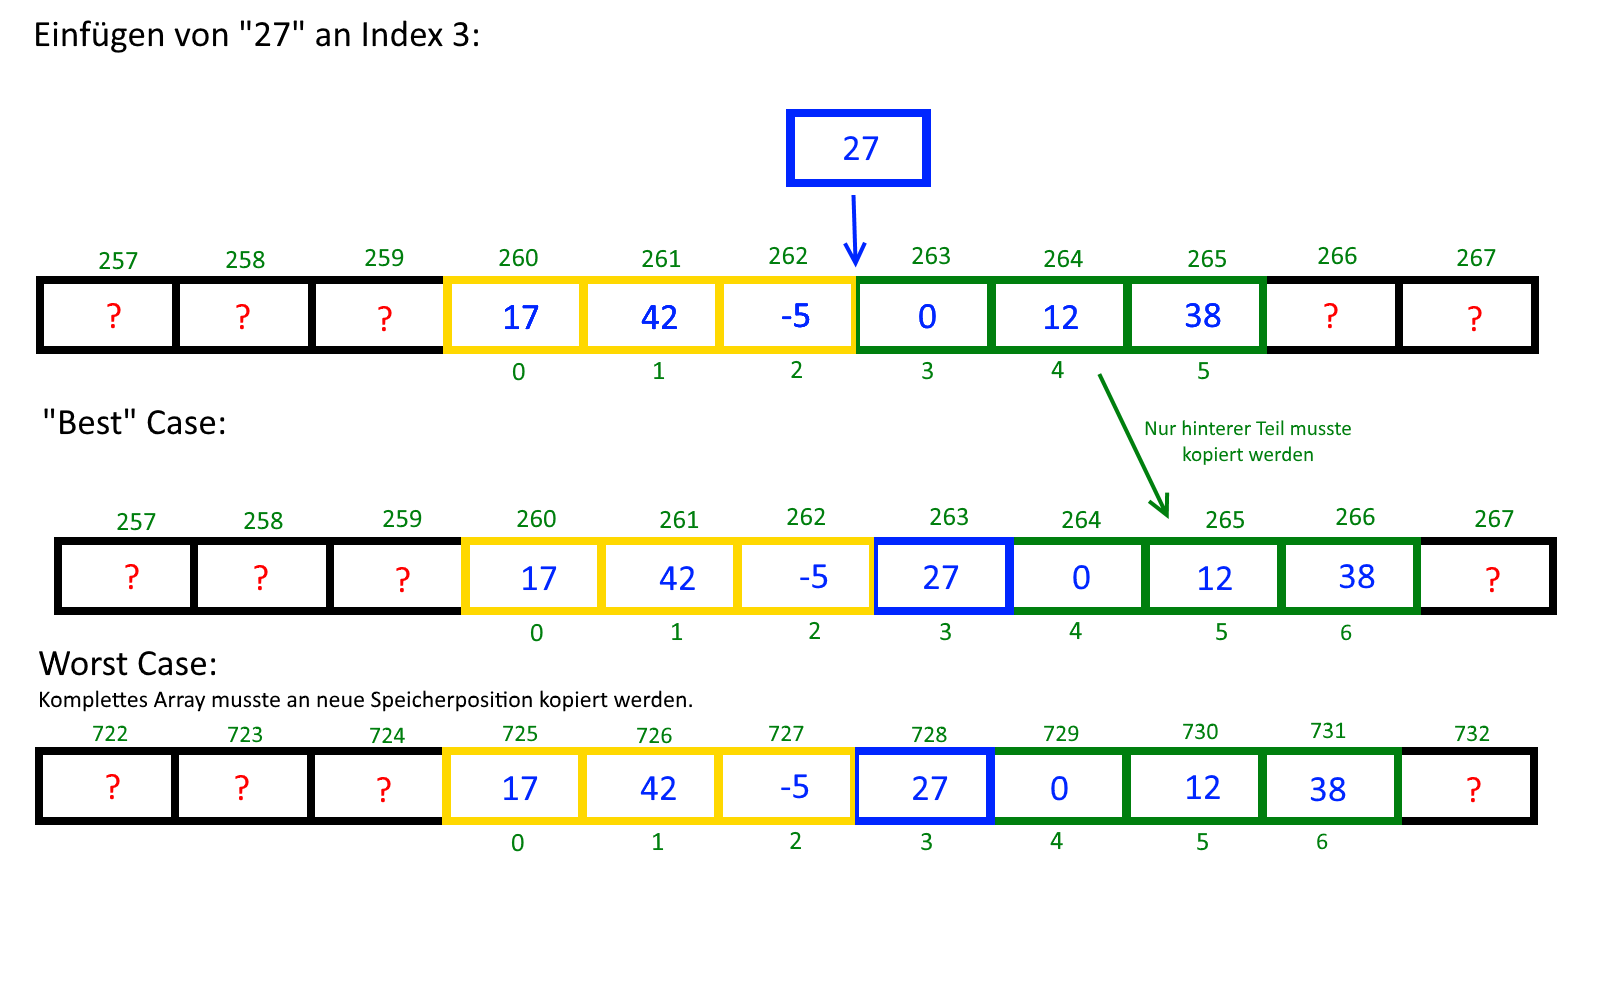
\includegraphics[height=6cm]{graph/array_insert}
\end{frame}

\begin{frame}{Komplexität}{Beim einfügen}
	\begin{itemize}
		\item Theoretischer Best-Case:
		\begin{itemize}
			\item Einfügen am Ende des Arrays
			\item ...solange der nachfolgende Speicher noch ungenutzt ist
			\item Dann wäre lediglich eine Kopieroperation erforderlich
		\end{itemize}
		\item In der Regel kann jedoch davon ausgegangen werden, dass...
		\begin{itemize}
			\item ...ein neues Array (an einem anderen Speicherbereich) angelegt werden muss
			\item ...und jedes Element des Arrays kopiert werden muss
		\end{itemize}
		\item Komplexität ergibt sich hierbei zu: $O(N)$
	\end{itemize}
\end{frame}

\begin{frame}{Ermitteln der Länge}{In Arrays}
	\begin{itemize}
		\item Bestimmen der Elemente eines Arrays nicht trivial möglich
		\item Da Array nur einen Speicherbereich beschreibt und seine eigene Größe nicht kennt
		\item Zählen von Elementen nicht möglich, da Abbruchbedingung nicht bekannt
		\item Größe muss somit selbst gespeichert und verwaltet werden
		\begin{itemize}
			\item Passiert in Java automatisch
			\item Da ein Array auch immer ein Objekt ist
			\item Bestimmen der Größe über das \texttt{length} Attribut
		\end{itemize}
	\end{itemize}
\end{frame}

\begin{frame}{Entfernen von Elementen}{In Arrays}
	\begin{itemize}
		\item Entfernen führt zu Problem im Speicherbereich:
		\item Durch das Entfernen würde eine "`Lücke"' im Array entstehen
		\item Daten im Array müssen jedoch fortlaufenden Speicher belegen
		\item D.h., Alle Elemente hinter dem entfernten Element müssen eine Position nach links verschoben werden
		\begin{itemize}
			\item "`Teure"' Kopiervorgänge nötig
		\end{itemize}
		\item Komplexität ergibt sich somit zu $O(N)$ (Worst-Case)
	\end{itemize}
\end{frame}

\begin{frame}{Entfernen von Elementen}{Visualisiert}
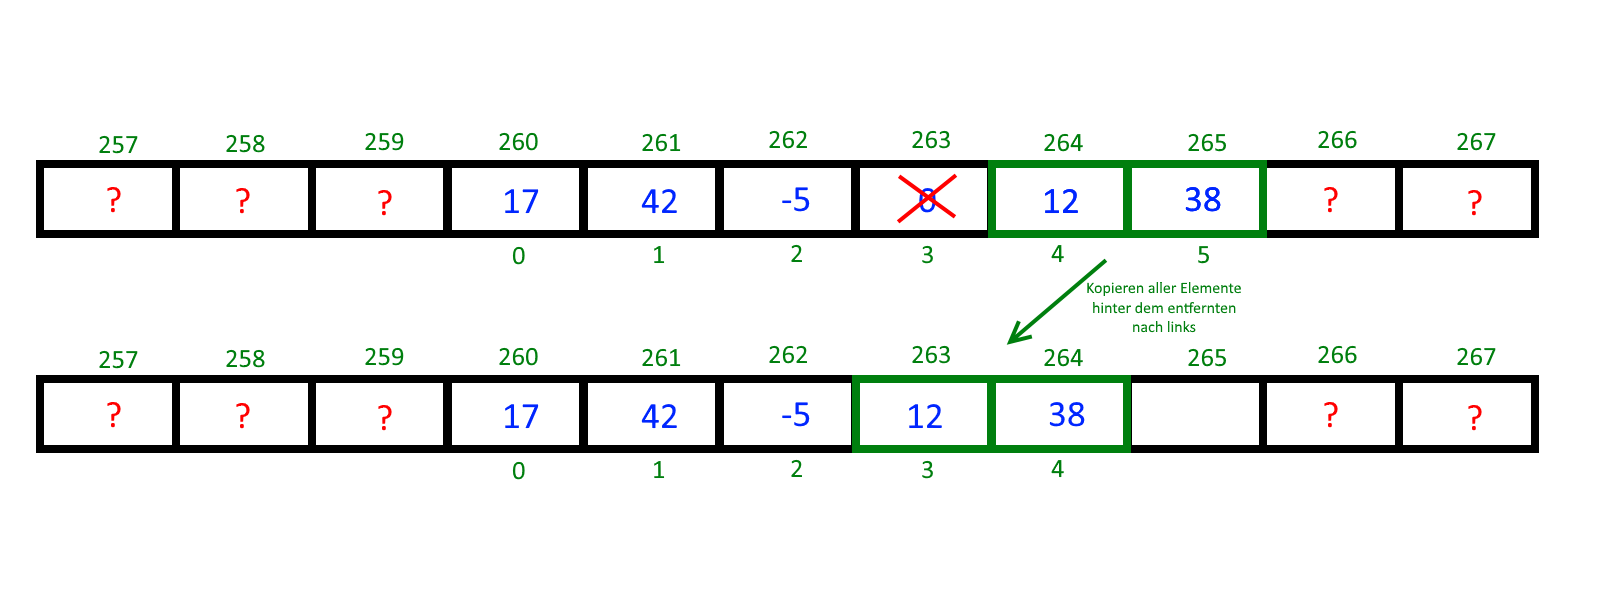
\includegraphics[width=\textwidth]{graph/array_remove}
\end{frame}

\begin{frame}{Entfernen von Elementen}{Weitere Aspekte}
	\begin{itemize}
		\item Beim entfernen von Elementen wird hinten Speicher "`frei"'
		\item Dieser ist (technisch) noch dem Array zugeordnet
		\begin{itemize}
			\item Heißt: Größe des Arrays muss theoretisch aktualisiert werden (Wenn man diese manuell verwalten muss)
		\end{itemize}
		\item Freigewordener Speicher kann jedoch später wiederverwendet werden:
		\begin{itemize}
			\item Elemente können theoretisch hinzugefügt werden ohne, dass das Array vergrößert werden muss
			\item Dafür müssen dann jedoch zwei Werte getracked werden:
			\item Die reservierte Größe des Arrays
			\item Die aktuell genutzte Größe des Arrays
			\item \texttt{ArrayList} Implementierung arbeitet ähnlich
		\end{itemize}
	\end{itemize}
\end{frame}

\begin{frame}{Konkatinieren von Arrays}
	\begin{itemize}
		\item Beim kombinieren zweier Arrays ergibt sich ähnliches Problem wie beim Einfügen
		\item Array hat ggf. nicht genug Platz um Elemente von beiden Arrays aufzunehmen
		\item Daher sind meist folgende Schritte nötig um zwei Arrays mit Länge $N$ und $M$ zu kombinieren:
		\begin{itemize}
			\item Anlegen eines neues Arrays mit Größe $N+M$
			\item Kopieren aller Elemente des ersten Arrays in den vorderen Teil
			\item Kopieren aller Elemente des zweiten Arrays in den hinteren Teil
		\end{itemize}
		\item Dadurch ergibt sich die Komplexität zu $O(N+M)$ (inklusive Overhead für Anlegen des neuen Arrays)
	\end{itemize}
\end{frame}

%\begin{frame}{Vor- und Nachteile}
%\end{frame}
	
	\outlineFrame{Linked Lists}
	\begin{frame}{Allgemeines}{Über Linked Lists}
	\begin{itemize}
		\item Simple Listenstruktur
		\item Elemente können verteilt im Speicher liegen
		\item Jedes Element speichert einen Datenwert
		\item ...und eine Referenz zum Nachfolger
		\item Speichern mehrdimensionaler Daten theoretisch möglich
		\begin{itemize}
			\item Wenn der Datenwert auch wieder eine Linked List ist
			\item Zugriff allerdings weniger intuitiv als im Array
		\end{itemize}
	\end{itemize}
\end{frame}


\begin{frame}{Eigenschaften}{Von Linked Lists}
	\begin{itemize}
		\item Muss keinen fortlaufenden Teil im Speicher belegen
		\item Dadurch entfallen einige Nachteile des Arrays:
		\begin{itemize}
			\item Größe muss nicht bei Initialisierung bekannt sein
			\item Liste kann dynamisch wachsen bzw. schrumpfen (Ohne "`teuere"' Kopiervorgänge)
			\item Einfügen bzw. Entfernen ist schneller
		\end{itemize}
		\item Allerdings ist der Zugriff auf Elemente langsamer
	\end{itemize}
\end{frame}

\begin{frame}{Datenstruktur von Linked Lists}{Listenelemente}
	\begin{itemize}
		\item Jedes Element einer Linked List ist ein Objekt
		\item Jedes Objekt vom Typ \textit{ListElement} besteht aus:
		\begin{itemize}
			\item Einem Member das den Wert des aktuellen Elements speichert. Datentyp ist der Typ, den die Liste speichert (\texttt{Double}, \texttt{Integer} etc.)
			\item Einem Member welches das nächste Element (bzw. eine Referenz darauf) in der Liste repräsentiert. Datentyp ist hier \texttt{ListElement}
		\end{itemize}
		\item Gibt es kein nächstes Element in der Liste kann dies über ein spezielles \texttt{tail} Objekt oder eine \texttt{null} Referenz dargestellt werden
	\end{itemize}
\end{frame}

\begin{frame}{Datenstruktur von Linked Lists}{Liste}
	\begin{itemize}
		\item Die Liste vom Typ \texttt{LinkedList} besteht an sich lediglich aus:
		\begin{itemize}
			\item Einem Member \texttt{head}(Auch: \texttt{first}, \texttt{top} o.Ä.) vom Typ \texttt{ListElement}, welches das erste Element der Liste repräsentiert.
			\item Den für die Liste benötigten Operationen zum Zugriff und Manipulation von Listenelementen
		\end{itemize}
		\item Sollte die Liste leer sein, so ist \texttt{head} ein Verweis auf \texttt{null} oder ein spezielles Element, das das Ende einer Liste repräsentiert.
	\end{itemize}
\end{frame}

\begin{frame}{Datenstruktur von Linked Lists}{Visualisiert}
%TODO: Visualisierung LinkedLists
\end{frame}

\begin{frame}{Grundoperationen}{Anlegen einer Linked List}
	\begin{itemize}
		\item Bei Anlegen einer neuen Linked List wird diese als leere Liste initialisiert
		\item Anders als beim Array muss kein Speicher für die Listenelemente reserviert werden
		\item Das heißt, das \texttt{head} Element wird mit einer \texttt{null} Referenz initialisiert
		\item Das erste Element, das hinzugefügt wird, wird automatisch zum \texttt{head} Elemente der Liste
		\item Wird ein Element hinzugefügt, wird erst zum Zeitpunkt des Hinzufügens der Speicher für dieses Element reserviert
	\end{itemize}
\end{frame}

\begin{frame}{Grundoperationen}{Zugriff auf Elemente}
	\begin{itemize}
		\item Zugriff auf Elemente muss immer sequentiell vom \texttt{head} Element aus erfolgen
		\item Zugriff auf das $n$-te Element erfolgt durch wiederholtes Zugreifen auf das \texttt{next} Element
		\item Bedeutet:
		\begin{itemize}
			\item Je weiter hinten das gesuchte Element steht, desto mehr Operationen sind möglich
			\item Somit ergibt sich die Komplexität zu $O(N)$
		\end{itemize}
	\end{itemize}
\end{frame}

\begin{frame}[fragile]{Zugriff auf Listenelemente}{Mögliche Codeimplementierung}
\lstset{style=java}
\begin{lstlisting}
public T getElement(int index){
	ListElement res = head;
	for(int i=0;i<index;i++){
		res = res.getNext();
	}
	return res.getValue();
}
\end{lstlisting}
\end{frame}
	
	\outlineFrame{Double Linked Lists}
	
	\outlineFrame{Aufgaben I}
	
	\outlineFrame{Stacks}
	
	\outlineFrame{Queues}
	
	\outlineFrame{Trees}
    
	\outlineFrame{Aufgaben II}
    \printbibliographyframe
    
	\section*{Kontakt}
	\begin{frame}{Kontakt}{}
	\begin{itemize}
		\item E-Mail: \href{mailto:lukas.abelt@airbus.com}{lukas.abelt@airbus.com}
		\item GitHub: \url{https://www.github.com/LuAbelt}
		\item GitLab: \url{https://www.gitlab.com/LuAbelt}
		\item Telefon(Firma): 07545 - 8 8895
		\item Telegram: LuAbelt
	\end{itemize}
\end{frame}
	

\end{document}